\documentclass[12pt, a4paper]{article}

\usepackage{array}
\usepackage{amsmath}
\usepackage[portuguese]{babel}
\usepackage{chngpage}
\usepackage{float}
\usepackage[a4paper, margin=2cm]{geometry}
\usepackage{graphicx}
\usepackage{hyperref}
\usepackage{setspace}
\usepackage{xcolor}

\title{\Huge \textbf{Computação Gráfica \\ \Large Trabalho Prático -- Fase I}}
\date{2 de março 2025}
\author{Grupo 3}

\begin{document}

\begin{center}
    
\includegraphics[width=0.25\textwidth]{res/cover/EE-C.eps}
\end{center}

\chardef\_=`_
\onehalfspacing
\setlength{\parskip}{\baselineskip}
\setlength{\parindent}{0pt}
\def\arraystretch{1.5}

{\let\newpage\relax\maketitle}
\maketitle
\thispagestyle{empty}

\vspace*{\fill}

\begin{adjustwidth}{-2cm}{-2cm} % These values only need to be large enough to center the table
    \begin{center}
        \begin{tabular}{>{\centering}p{0.25\textwidth}
                        >{\centering}p{0.25\textwidth}
                        >{\centering}p{0.25\textwidth}
                        >{\centering\arraybackslash}p{0.25\textwidth}}
            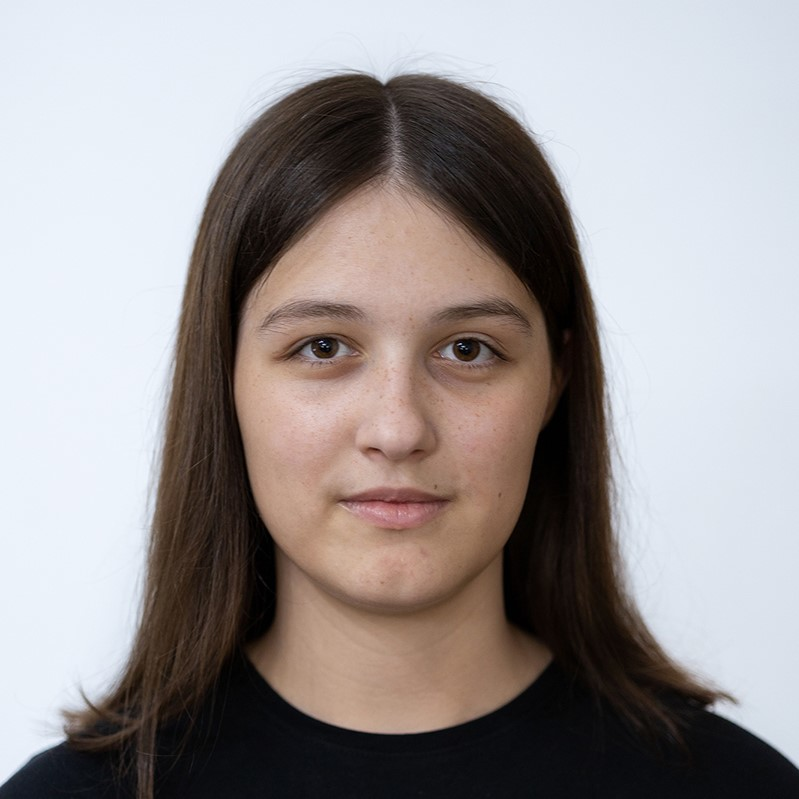
\includegraphics[width=3.5cm]{res/cover/A104437.png} &
            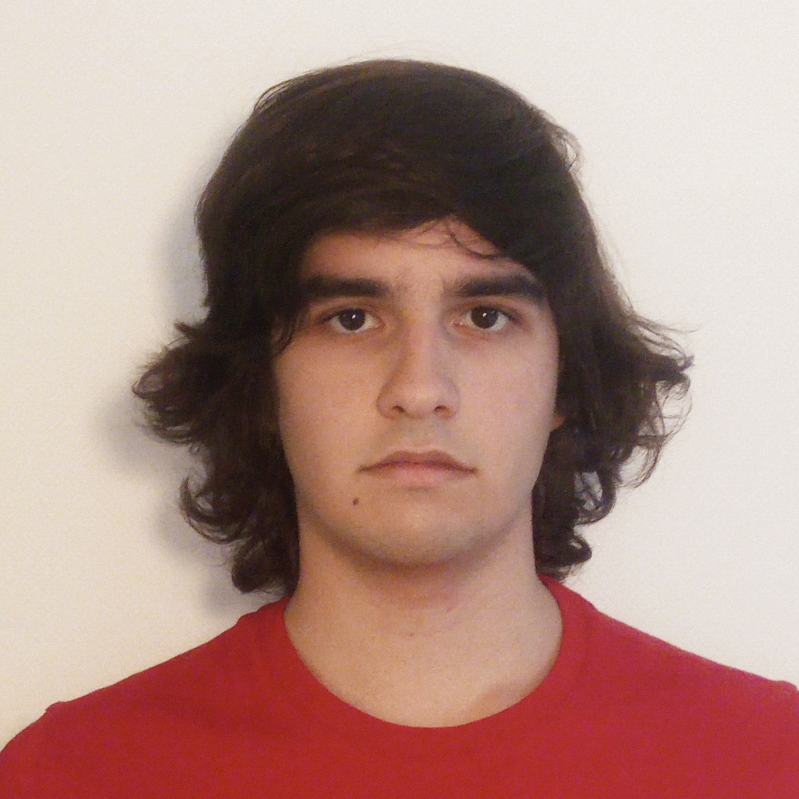
\includegraphics[width=3.5cm]{res/cover/A104348.png} &
            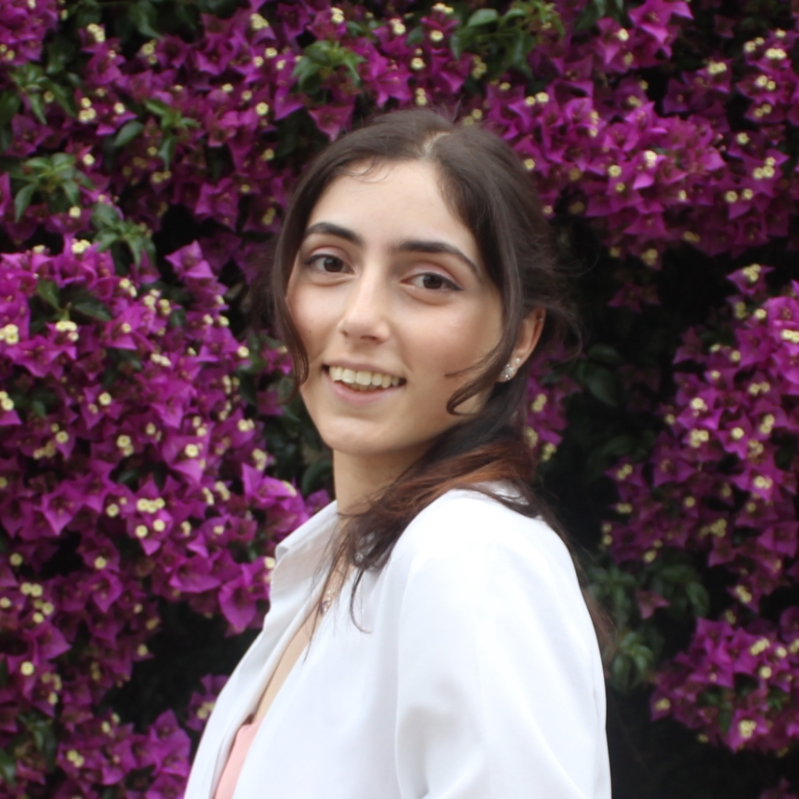
\includegraphics[width=3.5cm]{res/cover/A90817.png} &
            
\includegraphics[width=3.5cm]{res/cover/A104179.png} \\

            Ana Oliveira & Humberto Gomes & Mariana Cristino & Sara Lopes \\
            A104437      & A104348        & A90817           & A104179
        \end{tabular}
    \end{center}
\end{adjustwidth}

\pagebreak

\begin{abstract}
    \textbf{\color{red} TODO - resumo}
\end{abstract}

\section{\emph{Generator}}

\textbf{\color{red} TODO - \emph{generator}}

\subsection{Esfera}

Para construção da esfera, utilizámos um \textbf{sistema de coordenadas esféricas}, no qual a posição de cada ponto na esfera é
determinada por dois ângulos: o \textbf{ângulo polar} \( \theta \) e o \textbf{ângulo azimutal} \( \phi \).  

A parametrização de um ponto sobre uma esfera de raio \( r \) pode ser definida pelas seguintes equações:  
\[
x = r \sin(\theta) \cos(\phi)
\]
\[
y = r \cos(\theta)
\]
\[
z = r \sin(\theta) \sin(\phi)
\]
onde:
\begin{itemize}
\item \( \theta \) é o \textbf{ângulo polar}, que varia entre \( 0 \) (polo norte) e \( \pi \) (polo sul),
determina a latitude do ponto na esfera;  
\item \( \phi \) é o \textbf{ângulo azimutal}, que varia entre \( 0 \) e \( 2\pi \), define a longitude do
ponto.
\end{itemize}

Este modelo matemático permite gerar uma esfera distribuída no espaço tridimensional.
No entanto, para a sua implementação computacional, é necessário discretizar estes valores e definir um
conjunto finito de pontos e faces que aproximem à sua forma contínua.  

\subsubsection{Geração dos Vértices} 
Para discretizar a superfície da esfera, divide-se o intervalo de \( \theta \) em \textbf{stacks}
(fatias horizontais) e o intervalo de \( \phi \) em \textbf{slices} (segmentos verticais). Assim, as
incrementações angulares são calculados da seguinte forma:
\[
\Delta\theta = \frac{\pi}{\text{stacks}}, \quad \Delta\phi = \frac{2\pi}{\text{slices}}
\]
Ao percorrer os valores de \( \theta \) e \( \phi \), é possível gerar um conjunto ordenado de pontos
distribuídos sobre a esfera.  

De modo que, a construção dos vértices segue os seguintes passos:  

1. \textbf{Criação do pólo norte}: O primeiro ponto criado é o \textbf{pólo norte}, localizado em \( (0, r, 0) \).  

2. \textbf{Geração dos Pontos Intermédios}: Para cada \textbf{stack} (exceto as extremidades, que são os polos), iterámos sobre os valores de
   \( \theta \), determinámos a altura \( y \) do ponto e o raio da secção circular correspondente:
\[
y = r \cos(\theta)
\]
\[
r_{\text{secção}} = r \sin(\theta)
\]
Para cada \textbf{slice}, iterámos sobre os valores de \( \phi \), é calculada a posição dos pontos na
secção circular:
\[
x = r_{\text{secção}} \cos(\phi)
\]
\[
z = r_{\text{secção}} \sin(\phi)
\]

3. \textbf{Criação do pólo sul}: Após a geração das stacks intermédias, é criado o \textbf{pólo sul} em \( (0, -r, 0) \).   

\subsubsection{Construção das Faces}
Após a geração dos vértices, é necessário definir as faces triangulares que compõem a superfície esférica. A triangulação é realizada da seguinte forma:  

1. \textbf{Ligação ao pólo norte}: Cada ponto da primeira stack (exceto o pólo norte) forma um triângulo com o pólo norte e o ponto
seguinte na mesma stack. Para garantir continuidade circular, o último ponto da stack liga-se
novamente ao primeiro, ou seja, os vértices são ligados de forma a criar \textbf{duas faces
triangulares por célula}:
\[
T_1 = (P_1, P_3, P_2)
\]

\begin{figure}[H]
    \centering
    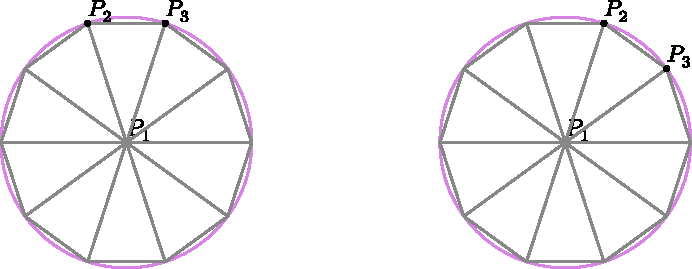
\includegraphics[width=0.4\textwidth]{res/figures/polos.pdf}
    \caption{
        Ilustração da ligação dos vértices da primeira stack ao pólo norte, formando os triângulos iniciais da esfera e a seguinte iteração.
    }
\end{figure}

2. \textbf{Ligação das stacks intermédias}:  
Para cada fatia horizontal da esfera, os vértices são ligados de forma a criar \textbf{duas faces
triangulares por célula}:
\[
T_1 = (P_1, P_3, P_4)
\]
\[
T_2 = (P_1, P_4, P_2)
\]

\begin{figure}[H]
    \centering
    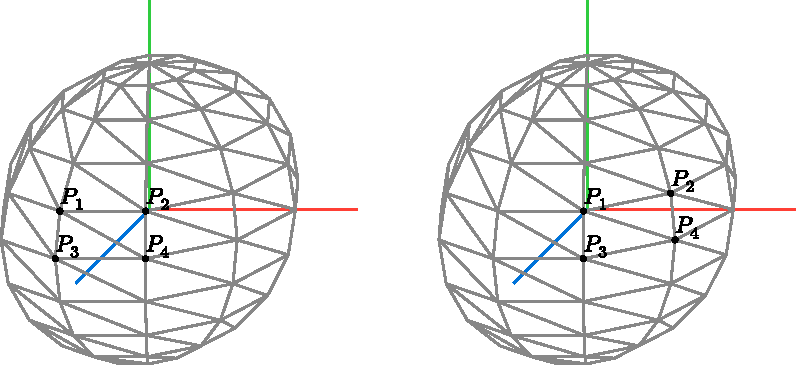
\includegraphics[width=0.4\textwidth]{res/figures/esferaIteration.pdf}
    \caption{
        Triângulos de uma esfera gerada, e pontos utilizados numa iteração do ciclo de geração
        de triângulos e na seguinte.
    }
\end{figure}

Este método assegura uma ligação contínua entre os pontos e evita a repetição de vértices
desnecessários.

3. \textbf{Ligação ao pólo sul}: O mesmo processo utilizado para o pólo norte é aplicado à stack mais
próxima do pólo sul, assim, garante que todas as fatias inferiores são corretamente ligadas ao vértice final.    

A ordenação dos vértices segue a \textbf{regra da orientação anti-horária}, permite a correta
aplicação da técnica de \textbf{face culling}, que otimiza o processo de renderização ao eliminar
automaticamente as faces voltadas para trás da câmara.  

Este método proporciona uma \textbf{representação eficiente e visualmente precisa}, garante uma
boa distribuição das faces ao longo da sua superfície.  

\section{\emph{Engine}}

\textbf{\color{red} TODO - \emph{engine}}

\section{Resultados obtidos}

\textbf{\color{red} TODO - resultados}

\section{Conclusão e Trabalho Futuro}

\textbf{\color{red} TODO - conclusão}

\begingroup
\section{Bibliografia}
\renewcommand{\section}[2]{}

\begin{thebibliography}{9}
    \bibitem{exemplo}
        \href{https://youtu.be/dQw4w9WgXcQ}{Um item de exemplo na bibliografia}
\end{thebibliography}
\endgroup

\end{document}
